\documentclass[11pt, a4paper]{article}
\usepackage[utf8]{inputenc}

\usepackage[margin=1in]{geometry} 
\usepackage{amsmath,amsthm,amssymb}
\usepackage[margin=1in]{geometry} 
\usepackage{amsmath,amsthm,amssymb}

\usepackage[slovene]{babel}
\usepackage{color}
\usepackage{graphicx}
\usepackage{amssymb}
\usepackage{amsmath}
\usepackage{mathtools}
\usepackage{commath}
\usepackage{ragged2e}
\usepackage[T1]{fontenc}
\usepackage[normalem]{ulem}
\usepackage{amsthm}
\usepackage{esvect}
\usepackage{float}
\usepackage{calrsfs}
\DeclareMathAlphabet{\pazocal}{OMS}{zplm}{m}{n}
\newcommand{\Ga}{\mathcal{G}}
\mathtoolsset{showonlyrefs} 

\newcommand\setItemnumber[1]{\setcounter{enumi}{\numexpr#1-1\relax}}


\newtheorem{theorem}{Trditev}[section]
\newtheorem{corollary}{Posledica}[section]
\newtheorem{lemma}[section]{Lema}
\theoremstyle{definition}
\newtheorem{definition}{Definicija}[section]
\theoremstyle{example}
\newtheorem{example}[section]{Primer}
\theoremstyle{izrek}
\newtheorem{izrek}[section]{Izrek}

\begin{document}
\begin{center}
\thispagestyle{empty}
\parskip=14pt%
\vspace*{3\parskip}%
\begin{Huge} Dielektricna anizotropija tekocega kristala \end{Huge}

By

Matic Tonin

ID No. (28181098)

Mentor 

(Rok Dolenec)

\rule{7cm}{0.4pt}

Pod okvirom:

FAKULTETE ZA FIZIKO IN MATEMATIKO, LJUBLJANA

13. 4. 2020

\end{center}
\pagebreak

\section{Naloga}
\begin{enumerate}

\item Izmerite temperaturno odvisnost komponent dielektricnega tenzorja vzdolž in pravokotno
na direktor.
\item Narišite na isti graf temperaturno odvisnost obeh komponent dielektricnega tenzorja
in povprecne dielektricne konstante. Narišite graf dielektricne anizotropije v
odvisnosti od temperature. Dolocite temperaturo faznega prehoda.
\item Izmerite odvisnost kapacitivnosti celice z orientacijo direktorja vzdolž stekelc od
napetosti, narišite graf C(U) ter dolocite elasticno konstanto tekocega kristala.
\end{enumerate}


\section{Meritve}
\subsection{Dielektricna anizotropija tekocega kristala}
Pri tej meritvi najprej postavimo vse aparature, kot nam kaže slika 4 v navodilih. Nas bo najbolj zanimala PT100 sonda, ki nam bo s pomočjo zveze med upornostjo in temperaturo povedala, kolikšna je temperatura v naši tekočekristalni celici. \\
PT100 je naziv za platinast uporovni termometer (angl. Resistance Temperature Detector RTD). Temperaturna
odvisnost upornosti je na intervalu [0,190 °C] opisana s formulo:
\begin{equation}
\label{Temperatura, upor}
R(T)= 100 \Omega(1+ 0.00385(T-273.16K)
\end{equation}
do 1\% natančno.\\

Na našem multimetru bomo merili kapacitivnost C in upornost R. Kapacitivbost merimo pri frekvenci 1kHz in amplitudo napetosi $U_{amp}=0.2$V. Pri tem pa potrebujemo upoštevati, da je kristal priklopljen na sinusno napetost, kristal pa se obnaša, kot bi bila nanj priklopljena enosmerna napetost z amplitudo.
\begin{equation}
\label{Sinusna-enosmerna napetost}
U_{RMS}= \frac{U_{AMP}}{\sqrt{2}}
\end{equation}

Preden pa začnemo izvajati meritev, potrebujemo izvedeti, kolikšna je kapacitivnost obeh tekočekristalnih celic pri sobni temperaturi, da vemo začetne točke grafa. Med merjenjem pa moramo paziti, da meritev ne izvajamo prehitro, saj se potrebuje temperatura ustaliti po celotnem vzorcu. Vse podatke o tem, pišejo v navodilih. Segrejemo pa ga do 65°C in ga nato ohlajamo ter zapisujemo kapacitivnosti C. \\

Za prazne celice so kapacitivnosti enake:

\begin{equation}
\label{Kapacitivnosti na praznem}
C_{\perp,0}=0.06nF \quad C_{||,0}=0.05nF
\end{equation}

Po znani teoriji in postopku dela se lotimo obdelave podatkov. 
Vemo, da se bo naša celica obnašala kot kondenzator in če zapišemo splošno formulu za kondenzator $C=\epsilon_0 \epsilon \frac{S}{d}$ lahko vidimo, da so vse ostale vrednosti, razen $\epsilon$, konstante. Tako lahko zapišemo, da je naš izmerjen $\epsilon$ za vsako temperaturo definiran kot:

\begin{equation}
\label{Dielektričnost}
\epsilon=\frac{C}{C_0}
\end{equation}
Kjer je $C_0$ kar kapacitovnost kondenzatorja pri prazni celici.Tako lahko sedaj izmerimo pri vsaki temperaturi našo vrednost $\epsilon_{\perp}$ in $\epsilon_{||}$. \\

Izmerjene meritve upora bomo najlažje napravili na grafu in sicer:

\begin{figure}[H]
	\centering
    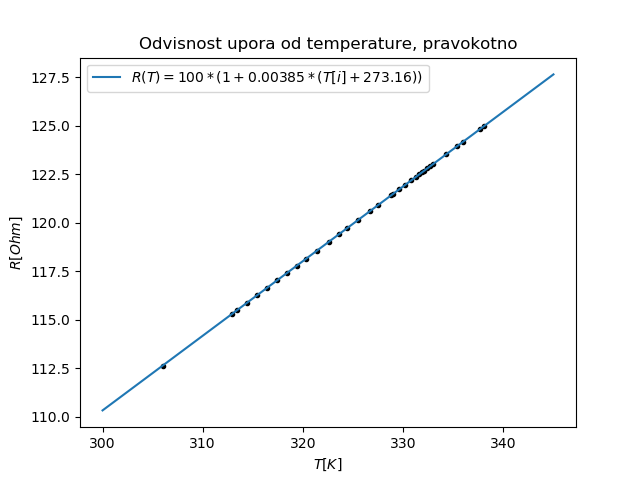
\includegraphics[width=12cm]{Upor_temperatura, pravokotno.png}
    \caption{Prikaz odvisnosti upora od temperature, pravokotno}
\end{figure}


\begin{figure}[H]
	\centering
    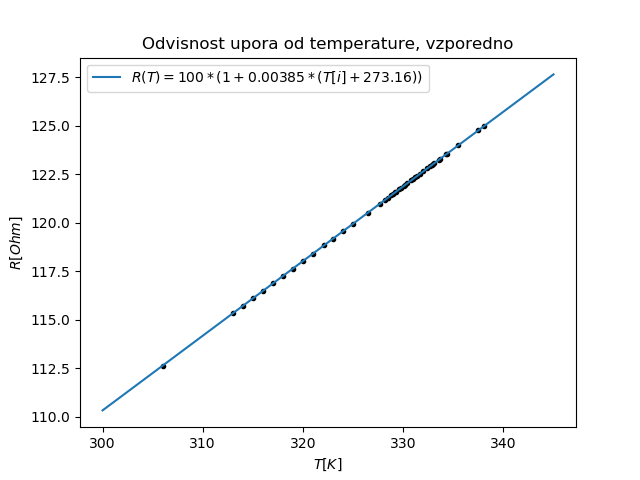
\includegraphics[width=12cm]{Upor_temperatura, vzporedno.png}
    \caption{Prikaz odvisnosti upora od temperature, vzporedno}
\end{figure}
Vidimo, da v obeh zvezah dobimo lepo linearno odvisnost, kot pričakovano. 
Če narišemo sedaj za vsak epsilon posebej, ne dobimo nič kaj dosti lepega, oz se nam odvisnost med eno in drugo vrednostjo ter kritična temperatura ne pokažeta dobro (posamična grafa lahko dodam na koncu vaje)
Če pa oba grafa rišemo na isti koorinatni sistem pa lahko dobimo temperaturo faznega prehoda, ki je ravno točka srečanja obeh grafov. Če sedaj narišemo ta graf in odčitamo vmesno točko, dobimo: 
\begin{figure}[H]
	\centering
    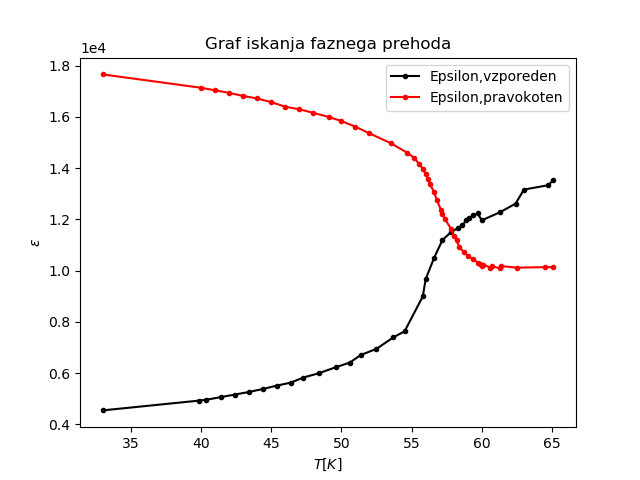
\includegraphics[width=12cm]{Fazni prehod.png}
    \caption{Prikaz odvisnosti obeh koeficientov dielektričnosti od temperature}
\end{figure}

Točke nam povejo, da se naša temperatura nahaja nekje v intervalu med:

$$ T[°C]= [57.2,58.4] $$

To vrednost smo poiskali tako, da smo naredili v našem programu pogoj, da če je razlika epsilonov v vzporedni in pravokotni smeri manjša od 500, naj nam vrne interval vrednosti temperature. Ta interval bi skrajšali, če bi naredili več meritev na tem območju. Sklepamo pa, da je pravilna temperatura neka vmesna temperatura, torej:

$$T=57.2 °C$$

Na grafu pa je razvidno tudi, da je v vzporedni dielektričnosti prišlo do neke zmede na grafu. Glavni razlog za to je verjetno, da so bile te meritve narejene naknadno in je bil zato koeficient čisto malo drugačen ali pa se je zgodila kakšna sistemska napaka za 4 meritve, saj se za naslednje meritve graf obnaša normalno. \\

Če sedaj še narišemo graf z povprečno dielektrično konstanto in razliko obeh konstant. Enačbi za za risanje pa sta: 

$$\overline{\epsilon}=\frac{2\epsilon_{\perp}+\epsilon_{||}}{3}$$
$$\Delta \epsilon=\epsilon_{||}-\epsilon_{\perp}$$

\begin{figure}[H]
	\centering
    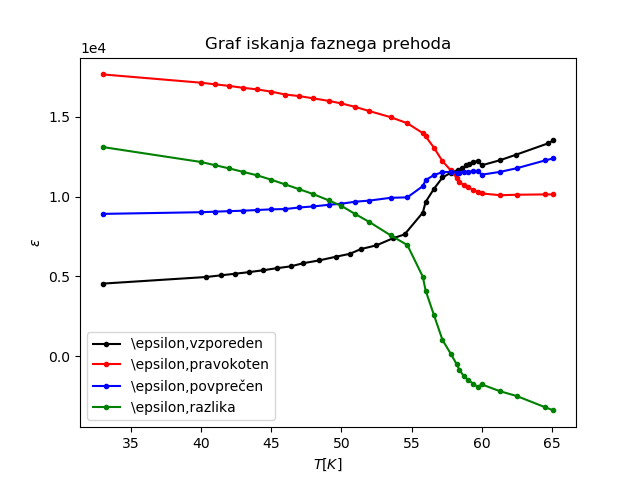
\includegraphics[width=12cm]{Povprečni epsilon.png}
    \caption{Prikaz vseh meritev epsilonov odvisnih od temperature}
\end{figure}

Vidimo, da je med faznim prehodom in po faznem prehodu prišlo do spremembe povprečnega epsilona, kar sklepamo, da je merska napaka, ki se nam pokaže že na grafu številka 3, kjer meritve $\epsilon_{||}$ hito poskočijo. En razlog bi lahko bil, da nismo počakali, da se temperatura pri faznem prehodu ustali. Torej da smo meritev izvajali prehitro, drugi pa, da je šlo kaj drugega narobe.  

\pagebreak

\subsection{Določanje temperature faznega prehoda preko grafa $\epsilon$}

Pri temperaturi faznega prehoda naj bi na grafu opazili nezveznost dielektrične anizotropije, a je v tem primeru težko določljiva, zato je težko natančno določiti temperaturo faznega prehoda. Če narišemo graf, ki ga opazujemo: 

\begin{figure}[H]
	\centering
    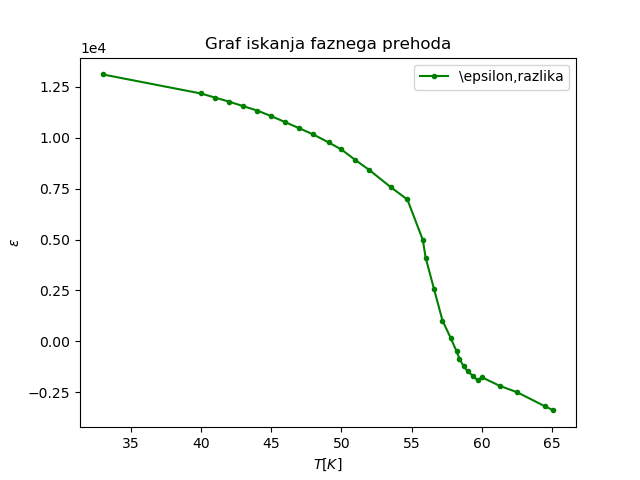
\includegraphics[width=10cm]{Fazni prehod,1.png}
    \caption{Prikaz vseh meritev epsilonov odvisnih od temperature}
\end{figure}

Če poskusimo najti interval, kjer bi se nahajal fazni prehod, dobimo, da je med:

$$T[C]=[57.5,59,5]$$

kar potrjuje tudi naša prejšnja slika.
\pagebreak
\subsection{Frederiksov prehod}
Sedaj imamo na mizi stojalo s celiko tekočega kristala površine 1cm x 1 cm in debeline $8 \mu m$. Površini sta prevodnu in dani na napetostni vir, vsaka celica pa ima na vsaki strani polarizator. Zato obstajata dve možnosti, ali da opazujemo dvolomnost v odvisnosti od električne napetosti na celici. Druga opcija pa je merjenje kapacitete celice v odvisnosti od napetosti in to bomo tudi počeli.\\
Najprej priklopimo celice, kot nam prikazuje slika v navodilih. Ker celica ni idealni kondenzator, slika na osciloskopu ne bo vedno elipsa, ampak se bomo približevali elipsi z višanjem frekvenc. Nastavimo tako, da je elipsa simetrična na x in y os.
Takrat je faza med tokom in napetostjo 90°. Določimo pa lahko kapaciteto kondenzatorja kot:

$$C=\frac{I_{AMP}}{\omega U_{AMP}}=\frac{U_R}{R \omega U_{AMP}}$$

V navodilih pa imamo znane podatke o R in $\omega$.
\begin{table}[h]
	\centering
	\begin{tabular}{|c|c|}
		\hline
		$R [\Omega]$ & $\omega [kHz] $ \\
		\hline
		\hline
		1000 & 100\\
		\hline
	\end{tabular}
	\caption{Podatki o naši aparaturi}		\label{osnove}
\end{table}
In ker smo že prej zapisali, da je kristal priklopljen na sinusno napetost, kristal pa se obnaša, kot bi bila nanj priklopljena enosmerna napetost z amplitudo, bomo sedaj upoštevali enačbo:
\begin{equation}
\label{Sinusna-enosmerna napetost}
U_{RMS}= \frac{U_{AMP}}{\sqrt{2}}
\end{equation}

Če narišemo sedaj graf odvisnosti kapacitivnosti od napetosti, dobimo, da je:\\

\begin{figure}[H]
	\centering
    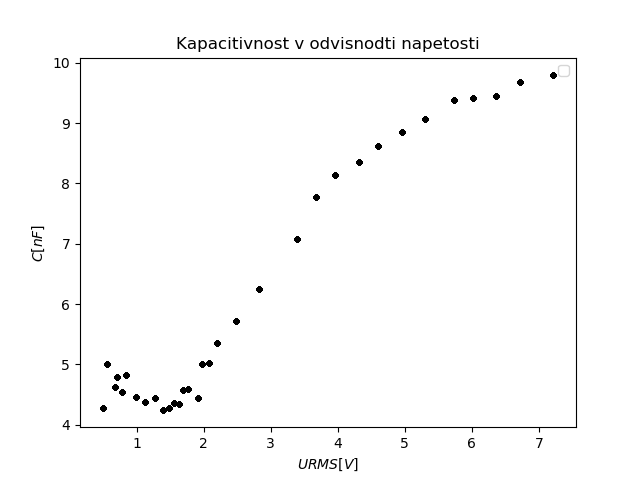
\includegraphics[width=12cm]{Kapacitivnost_napetost.png}
    \caption{Prikaz vseh meritev epsilonov odvisnih od temperature}
\end{figure}


Iz tega grafa pa lahko tudi razberemo, kdaj pride do Frederiksovega prehoda, ki se zgodi na intervalu:

$$U=[1.9, 1.95]V$$

Ker pa za izračun elastične konstante tekočih kristalov potrebujemo točno vrednost, pa lahko rečemo, da se zgodi približno na:

$$U_{crit}=1.92 V \pm 0.05 V$$
Za konec, pa lahko še določimo orientacijsko elastično konstanto tekočih kristalov $K_1$ in sicer iz enačbe: 

\begin{equation}
\label{Elastična konstanta}
K_1=\frac{U_{crit}^2 \Delta \epsilon \epsilon_0}{\pi^2}= (6.5 \pm 0.5)\cdot 10^{-12}\frac{kgm}{s^2}
\end{equation}

Za vrednosti naših $\Delta \epsilon $ vzamemo vrednost, iz prve metode, ko se zgodi fazni prehod. 
 



\end{document}